\documentclass{report}
\usepackage[T1]{fontenc} % Fontes T1
\usepackage[utf8]{inputenc} % Input UTF8
\usepackage[backend=biber, style=ieee]{biblatex} % para usar bibliografia
\usepackage{csquotes}
\usepackage[portuguese]{babel} %Usar língua portuguesa
\usepackage{blindtext} % Gerar texto automaticamente
\usepackage[printonlyused]{acronym}
\usepackage{hyperref} % para autoref
\usepackage{graphicx}
\usepackage{float}

\bibliography{bibliografia}


\begin{document}
%%
% Definições
%
\def\titulo{Adivinha o Número Secreto}
\def\data{30/05/2020}
\def\autores{Mauro Marques Canhão Filho, Patricia Rafaela da Rocha Cardoso }
\def\autorescontactos{(103411) mauro.filho@ua.pt, (103243) patriciarcardoso@ua.pt}
\def\versao{1.0}
\def\departamento{Departamento de Eletrônica, Telecomunicações e Informática (DETI)}
\def\empresa{Universidade de Aveiro}
\def\logotipo{ua.pdf}
%
%%%%%% CAPA %%%%%%
%
\renewcommand{\contentsname}{Índice}
\begin{titlepage}

\begin{center}
%
\vspace*{50mm}
%
{\Huge \titulo}\\ 
%
\vspace{10mm}
%
{\Large \empresa}\\
%
\vspace{10mm}
%
{\LARGE \autores}\\ 
%
\vspace{30mm}
%
\begin{figure}[h]
\center
\includegraphics{\logotipo}
\end{figure}
%
\vspace{30mm}
\end{center}
%
\begin{flushright}
\versao
\end{flushright}
\end{titlepage}

%%  Página de Título %%
\title{%
{\Huge\textbf{\titulo}}\\
{\Large \departamento\\ \empresa}
}
%
\author{%
    \autores \\
    \autorescontactos
}
%
\date{\data}
%
\maketitle

\pagenumbering{roman}

%%%%%% RESUMO %%%%%%
\begin{abstract}
Este relatório tem como objetivo descrever a implementação e a intereção entre um servidor e um ou mais clientes. Para isso, será detalhadamente apresentado o funcionamento/criação de um jogo. O jogo consiste em o cliente adivinhar um número inteiro aleatório entre 0 e 100, o número secreto, gerado aleatoriamente pelo servidor.
\end{abstract}

\tableofcontents
% \listoftables     % descomentar se necessário
% \listoffigures    % descomentar se necessário


%%%%%%%%%%%%%%%%%%%%%%%%%%%%%%%
\clearpage
\pagenumbering{arabic}

%%%%%%%%%%%%%%%%%%%%%%%%%%%%%%%%
\chapter{Introdução}
\label{chap.introducao}
O objetivo deste trabalho é explicar,enumerar e descrever o desenvolvimento e funcionamento de um servidor que suporte a geração de um número inteiro aleatório (entre 0 e 100), o número secreto, bem como o número máximo de tentativas (entre 10 e 30) concedidas para o adivinhar. E um cliente que permita adivinhar esse número secreto. Ou seja um jogo de adivinha o número secreto.
O servidor nunca deverá aceitar dois clientes com a mesma identificação a jogar simultaneamente e deverá criar e atualizar um ficheiro designado por report.csv onde vai escrevendo os resultados dos diversos clientes quando estes terminam o jogo. O cliente pode desistir em qualquer altura e o jogo acaba quando ele adivinha o número secreto ou quando esgota o número máximo de tentativas que dispunha para jogar. Caso o cliente exceda o número de jogadas de que dispunha o jogo será considerado sem sucesso mesmo que ele tenha adivinhado o número. Quando o jogo acaba corretamente o cliente deve escrever no monitor uma mensagem a indicar se adivinhou ou não o número secreto e quantas jogadas efectuou. Por sua vez o servidor acrescenta ao ficheiro a informação relativa ao jogo: cliente; número secreto; número máximo de jogadas; número de jogadas efectuadas; e o resultado obtido pelo cliente (desistência ou sucessso ou insucessso).

\chapter{Metodologia}
\label{chap.metodologia}
Neste capítulo será detalhadamente descrito o algoritmo e o funcionamento do progama servidor e do programa cliente bem como a implementação dos testes funcionais e unitários.
\section{Servidor}
O programa servidor consiste em gerar aleatoriamente um número entre 0 e 100 e um número máximo de tentativas entre 10 e 30 para o adivinhar. 
	O programa servidor é constítuido por um dicionário e as seguintes funções: \textbf{find\_client\_id},\textbf{encrypt\_intvalue}, \textbf{decrypt\_intvalue}, \textbf{new\_msg}, \textbf{numberToCompare}, \textbf{new\_client}, \textbf{clean\_client}, \textbf{quit\_client}, \textbf{create\_file}, \textbf{update\_file}, \textbf{guess\_client}, \textbf{stop\_client} e \textbf{main}.
\subsection{Dicionário e Array}
\begin{figure}[H]
	\centering
	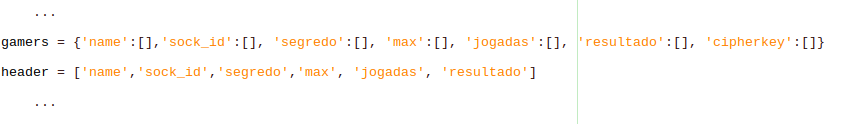
\includegraphics[scale=0.65]{dicionarioearray_server}	
	\caption{Dicionário constituído pelos dados dos jogadores e array responsável pela inicialização do header no ficheiro report.csv.}
\end{figure}

O dicionário "gamers" armazena os dados dos jogadores que estão atualmente com um jogo iniciado. A informação armazenada é baseada na ordem pela qual os clientes se conectam ao servidor. Essa informação é filtrada e distribuída por arrays que contém diferentes campos de identificação. Por exemplo, se dois jogadores, Mauro e Patrícia estiverem a jogar simultaneamente e se o Mauro se conectou primeiro ao servidor, o seu ID pode ser consultado através de: gamers['sock\_id'][0], enquanto o ID da Patrícia pode ser acedido da seguinte forma: gamers['sock\_id'][1].
O array "headers" é utilizado para atualizar o cabeçalho do ficheiro report.csv que será gerado pelo servidor.

\subsection{Função \textbf{find\_client\_id}}
\begin{figure}[H]
	\centering
	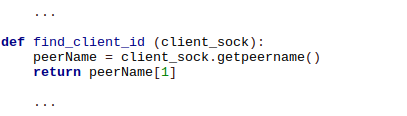
\includegraphics[scale=0.65]{find_client_id}	
	\caption{Função que retorna o porto ao qual o cliente está conectado.}

	A partir de cada socket de cliente, é possível extrair algumas informações únicas para o identificar.Neste caso, a função .getpeername() devolve uma sequência ordenada que contém o endereço do host e o porto ao qual o cliente está conectado. O porto, por sua vez, é devolvido pela função find\_client\_id().

\end{figure}
\subsection{Função \textbf{encrypt\_intvalue}}
\begin{figure}[H]
	\centering
	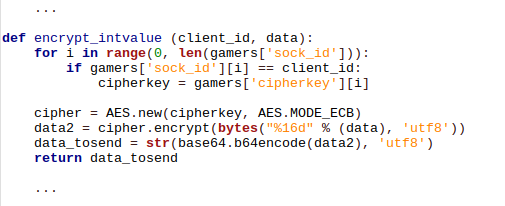
\includegraphics[scale=0.65]{encrypt_intvalue}	
	\caption{Função para encriptar valores a enviar em formato json com codificação base64.}
\end{figure}

Cada número inteiro comunicado entre o servidor e o cliente é encriptado por blocos usando a função AES-128 no modo ECB. A encriptação é realizada do seguinte modo: 
\begin{enumerate}
\item Identificação da chave de cifragem relativa ao cliente atual comparando o ID passado como argumento da função e os IDs presentes no dicionário "gamers";
\item Conversão do inteiro numa string binária de 128 bits;
\item Codificação da string no formato Base64 com o intuito dos criptogramas serem suportados pelo JSON;
\item Devolução pela função do valor codificado e encriptado para que possa ser enviado. 
\end{enumerate}

\subsection{Função \textbf{decrypt\_intvalue}}
\begin{figure}[H]
	\centering
	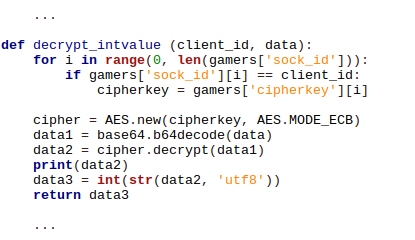
\includegraphics[scale=0.65]{decrypt_intvalue}	
	\caption{Função para desencriptar valores recebidos em formato json com codificação base64}
\end{figure}

Cada número inteiro comunicado entre o servidor e o cliente é decriptado por blocos usando a função AES-128 em modo ECB. A decriptação ocorre do seguinte modo:
\begin{enumerate}
\item Identificação da chave de cifragem relativa ao cliente atual comparando o ID passado como argumento da função e os IDs presentes no dicionário "gamers";
\item Descodificação dos dados passados à função como argumento no formato Base64 e decriptação do seu conteúdo;
\item Codificação para um valor inteiro;
\item Devolução do valor inteiro pela função.
\end{enumerate}

\subsection{Função \textbf{new\_msg}}
\begin{figure}[H]
	\centering
	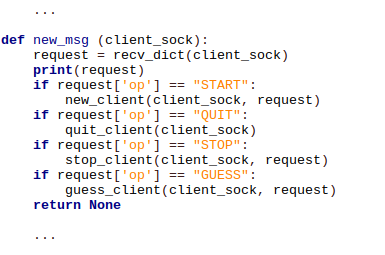
\includegraphics[scale=0.65]{new_msg}	
	\caption{Função chamada sempre que o servidor recebe uma nova mensagem do cliente.}
\end{figure}

A tarefa desta função é identificar qual a operação requisitada pelo cliente e encaminhá-la para a função que irá processar e responder ao pedido.
Caso seja feito um pedido de uma operação fora do alcançe da aplicação não ocorre qualquer comportamento por parte do servidor.

\subsection{Função \textbf{numberToCompare}}
\begin{figure}[H]
	\centering
	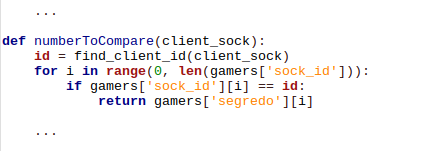
\includegraphics[scale=0.65]{numberToCompare}	
	\caption{Função que devolve o número secreto.}
\end{figure}

Esta função suporta o comando "Guess".

\subsection{Função \textbf{new\_client}}
\begin{figure}[H]
	\centering
	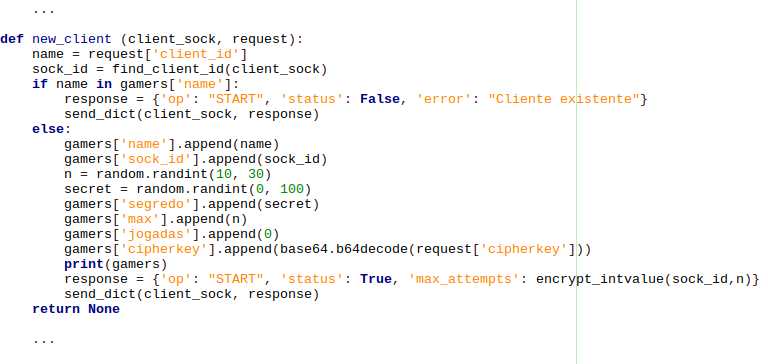
\includegraphics[scale=0.65]{new_client}	
	\caption{Função que cria um novo cliente no jogo.}
\end{figure}

Esta função suporta a criação de um novo jogador induzida pela operação START. O seu funcionamento pode ser descrito da seguinte forma: 
\begin{enumerate}
\item Armazenamento na variável "name" do "client\_id" passado para o servidor aquando da inserção pelo utilizador na linha de comandos ao executar o cliente;
\item Identificação do ID(porto ao qual está conectado) do cliente a partir do socket com a função "find\_client\_id";
\item Envio de uma resposta do servidor para o cliente com status: True; e com o valor encriptado de jogadas máximas que o cliente pode fazer.
\end{enumerate}
Se "name"("client\_id" enviado pelo pedido do cliente) já se encontre no dicionário "gamers", o servidor irá relatar ao cliente uma mensagem de status: False; e uma mensagem de erro indicando a já utilização desse nome.
Caso contrário, a função adiciona todos os dados necessários do cliente aos arrays do dicionário. É depois, iniciado um jogo.

\subsection{Função \textbf{clean\_client}}
\begin{figure}[H]
	\centering
	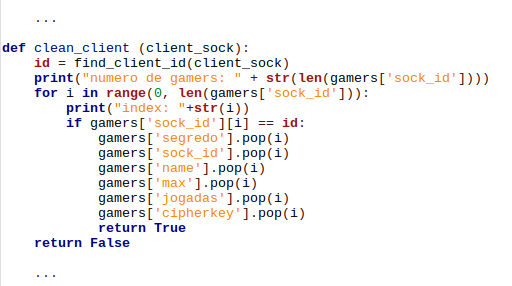
\includegraphics[scale=0.65]{clean_client}	
	\caption{Função chamada sempre que é necessário apagar um jogador da lista de jogadores ativos.}
\end{figure}

Esta função é executada sempre que for necessário excluir um cliente do dicionário "gamers". Isto ocorre quando o cliente se desconecta do servidor, quando termina o jogo ou quando desiste.
A função procura pelo cliente no dicionário "gamers" e caso o encontre, exclui todos os dados a ele associados através do seu respetivo índice.

\subsection{Função \textbf{quit\_client}}
\begin{figure}[H]
	\centering
	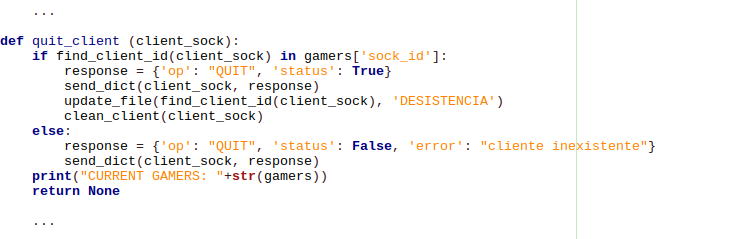
\includegraphics[scale=0.65]{quit_client}	
	\caption{Função chamada quando o cliente pretende desistir do jogo.}
\end{figure}

Esta função suporta o pedido de desistência de um cliente - operação QUIT.Primeiro, a função verifica se o cliente que pretende desistir encontra-se realmente em jogo. Para isto, verifica se o ID do socket está presente no dicionário "gamers".
Em caso afirmativo, o servidor envia uma mensagem ao cliente com status: True; e atualiza o ficheiro report.csv(recorrendo à função update\_file()) com o resultado "DESISTENCIA". Este resultado indica que a partida foi terminada antes de o jogador adivinhar o número secreto ou antes de atingir o limite de jogadas. Por fim, remove o cliente da lista de jogadores ativos recorrendo à função clean\_client.
Caso contrário, envia uma mensagem ao cliente com status: False; e uma mensagem de erro que explicita o facto de o cliente não ter sido encontrado entre os jogadores ativos.

\subsection{Função \textbf{create\_file}}
\begin{figure}[H]
	\centering
	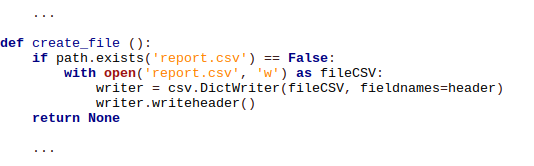
\includegraphics[scale=0.65]{create_file}	
	\caption{Função que cria um ficheiro report.csv quando o servidor é inicializado.}
\end{figure}

No momento em que o servidor é inicializado é chamada a função "create\_file" para que seja criado um novo ficheiro report.csv caso ainda não exista no diretório em que o server.py se encontra de maneira a que o servidor não reinicie o ficheiro toda a vez que for inicializado. Depois, escrever o cabeçalho no ficheiro com base no array "header".

\subsection{Função \textbf{update\_file}}
\begin{figure}[H]
	\centering
	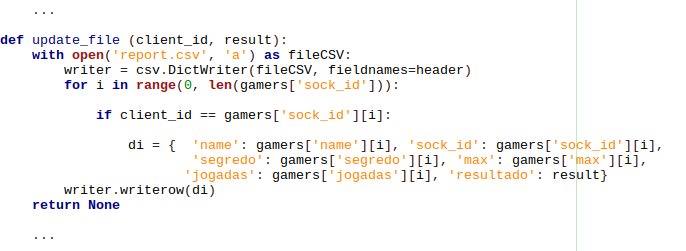
\includegraphics[scale=0.65]{update_file}	
	\caption{Função que atualiza o ficheiro report.csv quando um jogo é terminado.}
\end{figure}

Esta função atualiza o ficheiro report.csv com os dados de um jogador quando um jogo é terminado(com sucesso, sem sucesso ou desistência). Para isso, abre o ficheiro no modo "a"(append) para adicionar dados sem escrever sobre aqueles que já lá estavam.Assim, procura pelo index "i" tal que o sock\_id é igual ao client\_id passado como parâmetro da função. Por fim, escreve todos os itens na posição "i" dos arrays do dicionário "gamers". 

\subsection{Função \textbf{guess\_client}}
\begin{figure}[H]
	\centering
	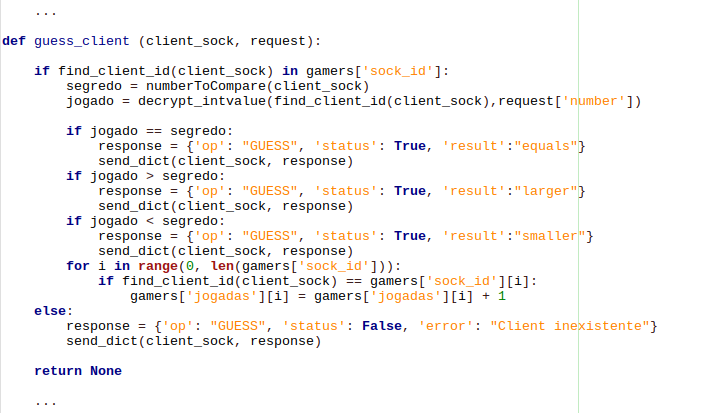
\includegraphics[scale=0.65]{guess_client}	
	\caption{Suporte da jogada de um cliente - Operação GUESS.}
\end{figure}

Para que a função possa funcionar corretamente, temos que averigurar se o cliente que está a jogar tem realmente uma sessão iniciada no jogo. Se ele se encontrar no dicionário "gamers" prosseguimos com o GUESS.Caso contrário, o servidor envia uma mensagem ao cliente com o status: False; e uma mensagem de erro a indicar que o cliente não se encontra na lista de jogadores ativos.
Consideremos agora o caso em que o cliente tem um jogo iniciado. Primeiro, procuramos o valor do número secreto deste cliente através da função "numberToCompare()", que será armazenado na variável segredo. Depois, descriptografamos o número inserido pelo jogador(que é passado na mensagem enviada do cliente ao servidor e que depois é encaminhada para a função pelo parâmetro "request") que é armazenado na variável "jogado".
Se o número for igual ao número secreto, o servidor envia uma mensagem ao cliente com status: True e result: "equals", a indicar que o jogador acertou no número.
Se o número for maior que o segredo, o servidor envia uma mensagem ao cliente com status: True e result: "larger" a indicar que o jogador introduziu um número superior ao número secreto.
Se o número for menor que o segredo, o servidor envia uma mensagem ao cliente com status: True e result: "smaller", a indicar que o jogador introduziu um número mais pequeno que o número secreto.
Por fim, atualiza no dicionário "gamers" o número de jogadas efetuadas.

\subsection{Função \textbf{stop\_client}}
\begin{figure}[H]
	\centering
	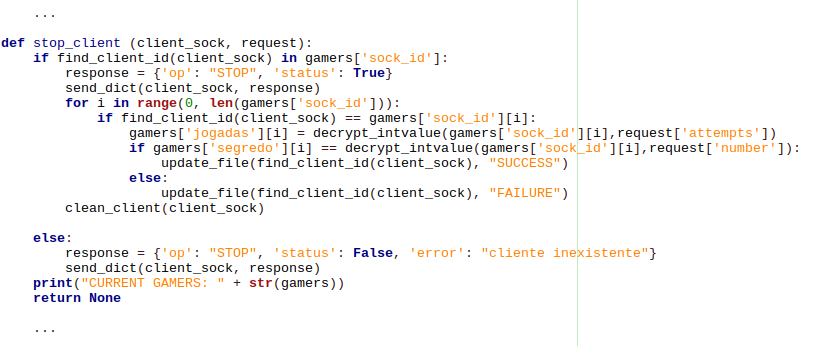
\includegraphics[scale=0.65]{stop_client}	
	\caption{Função responsável por encerrar o jogo.}
\end{figure}

Representa o suporte do pedido de terminação de um cliente - a operação STOP.
Esta operação ocorre sempre que um jogo é terminado ou porque o jogador acertou no número secreto ou porque efetuou mais jogadas dos que as que possuía.
Para que um jogo seja encerrado, o cliente precisa estar na lista de jogadores ativos, ou seja, no dicionário "gamers".
Se o cliente não se encontrar ativo no jogo, a função envia-lhe uma mensagem com status: False e uma mensagem de erro a indicar que o cliente não se encontra na lista de jogadores ativos.
Caso o cliente esteja ativo no jogo, o servidor envia-lhe uma mensagem com status: True, a indicar que a finalização do jogo foi processada.
O processamento do encerramento do jogo dá-se da seguinte forma: 
\begin{enumerate}
\item O servidor atualiza no dicionário "gamers" o número de jogadas efetuadas pelo jogador. Para isso, deve descriptograr o número inteiro enviado pelo cliente com auxílio da função "decrypt\_intvalue()";
\item O servidor verifica se o último número jogado pelo utilizador(que também deve ser descriptografado) coincide com o número secreto.
Caso seja, atualiza o ficheiro report.csv com os dados do cliente e o resultado final "SUCCESS". Caso contrário, atualiza o ficheiro report.csv com os dados do cliente e o resultado final "FAILURE";
\item Elimina o cliente da lista de jogadores ativos através da função "clean\_client()".
\end{enumerate}


\subsection{Função \textbf{main}}
\begin{figure}[H]
	\centering
	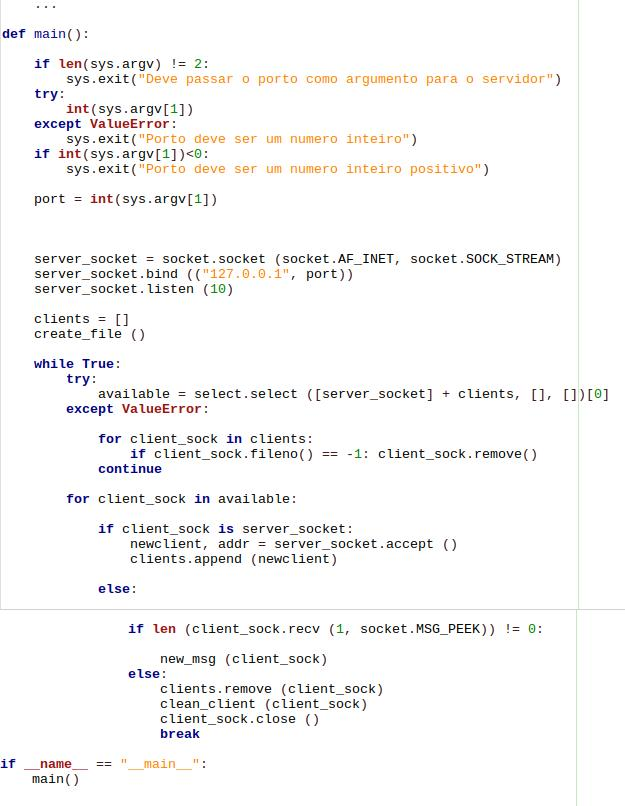
\includegraphics[scale=0.65]{main}	
	\caption{Função que permite o funcionamento correto de todo o servidor.}
\end{figure}

\section{Cliente}



\chapter{Resultados}
\label{chap.resultados}

\chapter{Análise}
\label{chap.analise}


\chapter{Conclusões}
\label{chap.conclusao}

\chapter*{Contribuições dos autores}


%%%%%%%%%%%%%%%%%%%%%%%%%%%%%%%%%
\chapter*{Acrónimos}


%%%%%%%%%%%%%%%%%%%%%%%%%%%%%%%%%
\printbibliography

\end{document}
